\documentclass[11pt,letterpaper]{article}

% Build steps (from this folder):
% 1) pdflatex Module5.tex
% 2) makeglossaries Module5
% 3) pdflatex Module5.tex
% 4) pdflatex Module5.tex

% ── Packages ──────────────────────────────────────────────────
\usepackage[margin=1in]{geometry}
\usepackage{titlesec}
\usepackage{enumitem}
\usepackage{booktabs}
\usepackage{tabularx}
\usepackage{graphicx}
\usepackage{xcolor}
\usepackage{hyperref}
\usepackage{fancyhdr}
\usepackage{amsmath}
\usepackage{amssymb}
\usepackage{tcolorbox}
\usepackage{multicol}
\usepackage{caption}
\usepackage{tikz}
\usepackage{listings}
\usepackage[acronym,toc,nopostdot]{glossaries}
\usetikzlibrary{shapes.geometric, arrows.meta, positioning, fit, calc, decorations.pathreplacing}
\makenoidxglossaries%
% Shared acronym macro container for EE800/820 lesson plan modules.
% Usage: type \IDE, \FPGA, \UART, etc. First use is expanded; later uses show acronym only.
% Requires in each document preamble:
%   \usepackage[acronym,toc]{glossaries}
%   \makeglossaries
%   % Shared acronym macro container for EE800/820 lesson plan modules.
% Usage: type \IDE, \FPGA, \UART, etc. First use is expanded; later uses show acronym only.
% Requires in each document preamble:
%   \usepackage[acronym,toc]{glossaries}
%   \makeglossaries
%   % Shared acronym macro container for EE800/820 lesson plan modules.
% Usage: type \IDE, \FPGA, \UART, etc. First use is expanded; later uses show acronym only.
% Requires in each document preamble:
%   \usepackage[acronym,toc]{glossaries}
%   \makeglossaries
%   \input{../glossary}
% Print used acronyms near end of document:
%   \printglossary[type=\acronymtype,title={Acronyms Used}]

% Acronym definitions (only used entries appear in the printed glossary).
\newacronym{ask}{ASK}{Amplitude Shift Keying}
\newacronym{bga}{BGA}{Ball Grid Array}
\newacronym{bom}{BOM}{Bill of Materials}
\newacronym{bram}{BRAM}{Block Random Access Memory}
\newacronym{crc}{CRC}{Cyclic Redundancy Check}
\newacronym{css}{CSS}{Chirp Spread Spectrum}
\newacronym{dma}{DMA}{Direct Memory Access}
\newacronym{dsp}{DSP}{Digital Signal Processing}
\newacronym{eda}{EDA}{Exploratory Data Analysis}
\newacronym{fifo}{FIFO}{First In, First Out}
\newacronym{fpga}{FPGA}{Field-Programmable Gate Array}
\newacronym{fsk}{FSK}{Frequency Shift Keying}
\newacronym{fsm}{FSM}{Finite State Machine}
\newacronym{gpio}{GPIO}{General-Purpose Input/Output}
\newacronym{hal}{HAL}{Hardware Abstraction Layer}
\newacronym{i2c}{I\textsuperscript{2}C}{Inter-Integrated Circuit}
\newacronym{ide}{IDE}{Integrated Development Environment}
\newacronym{ila}{ILA}{Integrated Logic Analyzer}
\newacronym{ism}{ISM}{Industrial, Scientific, and Medical}
\newacronym{isr}{ISR}{Interrupt Service Routine}
\newacronym{lut}{LUT}{Look-Up Table}
\newacronym{mcu}{MCU}{Microcontroller Unit}
\newacronym{ml}{ML}{Machine Learning}
\newacronym{ook}{OOK}{On-Off Keying}
\newacronym{per}{PER}{Packet Error Rate}
\newacronym{rf}{RF}{Radio Frequency}
\newacronym{rssi}{RSSI}{Received Signal Strength Indicator}
\newacronym{rtl}{RTL}{Register-Transfer Level}
\newacronym{snr}{SNR}{Signal-to-Noise Ratio}
\newacronym{spi}{SPI}{Serial Peripheral Interface}
\newacronym{uart}{UART}{Universal Asynchronous Receiver/Transmitter}
\newacronym{vhdl}{VHDL}{VHSIC Hardware Description Language}

% Convenience wrappers so you can type \IDE, \RF, etc.
\providecommand{\ASK}{\gls{ask}}
\providecommand{\BGA}{\gls{bga}}
\providecommand{\BOM}{\gls{bom}}
\providecommand{\BRAM}{\gls{bram}}
\providecommand{\CRC}{\gls{crc}}
\providecommand{\CSS}{\gls{css}}
\providecommand{\DMA}{\gls{dma}}
\providecommand{\DSP}{\gls{dsp}}
\providecommand{\EDA}{\gls{eda}}
\providecommand{\FIFO}{\gls{fifo}}
\providecommand{\FPGA}{\gls{fpga}}
\providecommand{\FSK}{\gls{fsk}}
\providecommand{\FSM}{\gls{fsm}}
\providecommand{\GPIO}{\gls{gpio}}
\providecommand{\HAL}{\gls{hal}}
\providecommand{\IIC}{\gls{i2c}}
\providecommand{\IDE}{\gls{ide}}
\providecommand{\ILA}{\gls{ila}}
\providecommand{\ISM}{\gls{ism}}
\providecommand{\ISR}{\gls{isr}}
\providecommand{\LUT}{\gls{lut}}
\providecommand{\MCU}{\gls{mcu}}
\providecommand{\ML}{\gls{ml}}
\providecommand{\OOK}{\gls{ook}}
\providecommand{\PER}{\gls{per}}
\providecommand{\RF}{\gls{rf}}
\providecommand{\RSSI}{\gls{rssi}}
\providecommand{\RTL}{\gls{rtl}}
\providecommand{\SNR}{\gls{snr}}
\providecommand{\SPI}{\gls{spi}}
\providecommand{\UART}{\gls{uart}}
\providecommand{\VHDL}{\gls{vhdl}}


% Print used acronyms near end of document:
%   \printglossary[type=\acronymtype,title={Acronyms Used}]

% Acronym definitions (only used entries appear in the printed glossary).
\newacronym{ask}{ASK}{Amplitude Shift Keying}
\newacronym{bga}{BGA}{Ball Grid Array}
\newacronym{bom}{BOM}{Bill of Materials}
\newacronym{bram}{BRAM}{Block Random Access Memory}
\newacronym{crc}{CRC}{Cyclic Redundancy Check}
\newacronym{css}{CSS}{Chirp Spread Spectrum}
\newacronym{dma}{DMA}{Direct Memory Access}
\newacronym{dsp}{DSP}{Digital Signal Processing}
\newacronym{eda}{EDA}{Exploratory Data Analysis}
\newacronym{fifo}{FIFO}{First In, First Out}
\newacronym{fpga}{FPGA}{Field-Programmable Gate Array}
\newacronym{fsk}{FSK}{Frequency Shift Keying}
\newacronym{fsm}{FSM}{Finite State Machine}
\newacronym{gpio}{GPIO}{General-Purpose Input/Output}
\newacronym{hal}{HAL}{Hardware Abstraction Layer}
\newacronym{i2c}{I\textsuperscript{2}C}{Inter-Integrated Circuit}
\newacronym{ide}{IDE}{Integrated Development Environment}
\newacronym{ila}{ILA}{Integrated Logic Analyzer}
\newacronym{ism}{ISM}{Industrial, Scientific, and Medical}
\newacronym{isr}{ISR}{Interrupt Service Routine}
\newacronym{lut}{LUT}{Look-Up Table}
\newacronym{mcu}{MCU}{Microcontroller Unit}
\newacronym{ml}{ML}{Machine Learning}
\newacronym{ook}{OOK}{On-Off Keying}
\newacronym{per}{PER}{Packet Error Rate}
\newacronym{rf}{RF}{Radio Frequency}
\newacronym{rssi}{RSSI}{Received Signal Strength Indicator}
\newacronym{rtl}{RTL}{Register-Transfer Level}
\newacronym{snr}{SNR}{Signal-to-Noise Ratio}
\newacronym{spi}{SPI}{Serial Peripheral Interface}
\newacronym{uart}{UART}{Universal Asynchronous Receiver/Transmitter}
\newacronym{vhdl}{VHDL}{VHSIC Hardware Description Language}

% Convenience wrappers so you can type \IDE, \RF, etc.
\providecommand{\ASK}{\gls{ask}}
\providecommand{\BGA}{\gls{bga}}
\providecommand{\BOM}{\gls{bom}}
\providecommand{\BRAM}{\gls{bram}}
\providecommand{\CRC}{\gls{crc}}
\providecommand{\CSS}{\gls{css}}
\providecommand{\DMA}{\gls{dma}}
\providecommand{\DSP}{\gls{dsp}}
\providecommand{\EDA}{\gls{eda}}
\providecommand{\FIFO}{\gls{fifo}}
\providecommand{\FPGA}{\gls{fpga}}
\providecommand{\FSK}{\gls{fsk}}
\providecommand{\FSM}{\gls{fsm}}
\providecommand{\GPIO}{\gls{gpio}}
\providecommand{\HAL}{\gls{hal}}
\providecommand{\IIC}{\gls{i2c}}
\providecommand{\IDE}{\gls{ide}}
\providecommand{\ILA}{\gls{ila}}
\providecommand{\ISM}{\gls{ism}}
\providecommand{\ISR}{\gls{isr}}
\providecommand{\LUT}{\gls{lut}}
\providecommand{\MCU}{\gls{mcu}}
\providecommand{\ML}{\gls{ml}}
\providecommand{\OOK}{\gls{ook}}
\providecommand{\PER}{\gls{per}}
\providecommand{\RF}{\gls{rf}}
\providecommand{\RSSI}{\gls{rssi}}
\providecommand{\RTL}{\gls{rtl}}
\providecommand{\SNR}{\gls{snr}}
\providecommand{\SPI}{\gls{spi}}
\providecommand{\UART}{\gls{uart}}
\providecommand{\VHDL}{\gls{vhdl}}


% Print used acronyms near end of document:
%   \printglossary[type=\acronymtype,title={Acronyms Used}]

% Acronym definitions (only used entries appear in the printed glossary).
\newacronym{ask}{ASK}{Amplitude Shift Keying}
\newacronym{bga}{BGA}{Ball Grid Array}
\newacronym{bom}{BOM}{Bill of Materials}
\newacronym{bram}{BRAM}{Block Random Access Memory}
\newacronym{crc}{CRC}{Cyclic Redundancy Check}
\newacronym{css}{CSS}{Chirp Spread Spectrum}
\newacronym{dma}{DMA}{Direct Memory Access}
\newacronym{dsp}{DSP}{Digital Signal Processing}
\newacronym{eda}{EDA}{Exploratory Data Analysis}
\newacronym{fifo}{FIFO}{First In, First Out}
\newacronym{fpga}{FPGA}{Field-Programmable Gate Array}
\newacronym{fsk}{FSK}{Frequency Shift Keying}
\newacronym{fsm}{FSM}{Finite State Machine}
\newacronym{gpio}{GPIO}{General-Purpose Input/Output}
\newacronym{hal}{HAL}{Hardware Abstraction Layer}
\newacronym{i2c}{I\textsuperscript{2}C}{Inter-Integrated Circuit}
\newacronym{ide}{IDE}{Integrated Development Environment}
\newacronym{ila}{ILA}{Integrated Logic Analyzer}
\newacronym{ism}{ISM}{Industrial, Scientific, and Medical}
\newacronym{isr}{ISR}{Interrupt Service Routine}
\newacronym{lut}{LUT}{Look-Up Table}
\newacronym{mcu}{MCU}{Microcontroller Unit}
\newacronym{ml}{ML}{Machine Learning}
\newacronym{ook}{OOK}{On-Off Keying}
\newacronym{per}{PER}{Packet Error Rate}
\newacronym{rf}{RF}{Radio Frequency}
\newacronym{rssi}{RSSI}{Received Signal Strength Indicator}
\newacronym{rtl}{RTL}{Register-Transfer Level}
\newacronym{snr}{SNR}{Signal-to-Noise Ratio}
\newacronym{spi}{SPI}{Serial Peripheral Interface}
\newacronym{uart}{UART}{Universal Asynchronous Receiver/Transmitter}
\newacronym{vhdl}{VHDL}{VHSIC Hardware Description Language}

% Convenience wrappers so you can type \IDE, \RF, etc.
\providecommand{\ASK}{\gls{ask}}
\providecommand{\BGA}{\gls{bga}}
\providecommand{\BOM}{\gls{bom}}
\providecommand{\BRAM}{\gls{bram}}
\providecommand{\CRC}{\gls{crc}}
\providecommand{\CSS}{\gls{css}}
\providecommand{\DMA}{\gls{dma}}
\providecommand{\DSP}{\gls{dsp}}
\providecommand{\EDA}{\gls{eda}}
\providecommand{\FIFO}{\gls{fifo}}
\providecommand{\FPGA}{\gls{fpga}}
\providecommand{\FSK}{\gls{fsk}}
\providecommand{\FSM}{\gls{fsm}}
\providecommand{\GPIO}{\gls{gpio}}
\providecommand{\HAL}{\gls{hal}}
\providecommand{\IIC}{\gls{i2c}}
\providecommand{\IDE}{\gls{ide}}
\providecommand{\ILA}{\gls{ila}}
\providecommand{\ISM}{\gls{ism}}
\providecommand{\ISR}{\gls{isr}}
\providecommand{\LUT}{\gls{lut}}
\providecommand{\MCU}{\gls{mcu}}
\providecommand{\ML}{\gls{ml}}
\providecommand{\OOK}{\gls{ook}}
\providecommand{\PER}{\gls{per}}
\providecommand{\RF}{\gls{rf}}
\providecommand{\RSSI}{\gls{rssi}}
\providecommand{\RTL}{\gls{rtl}}
\providecommand{\SNR}{\gls{snr}}
\providecommand{\SPI}{\gls{spi}}
\providecommand{\UART}{\gls{uart}}
\providecommand{\VHDL}{\gls{vhdl}}



% ── Colors ────────────────────────────────────────────────────
\definecolor{stevens}{RGB}{163,31,52}       % Stevens Red
\definecolor{darkgray}{RGB}{60,60,60}
\definecolor{lightgray}{RGB}{240,240,240}
\definecolor{accentblue}{RGB}{30,80,140}

% ── Hyperref Setup ────────────────────────────────────────────
\hypersetup{
	colorlinks=true,
	linkcolor=stevens,
	urlcolor=accentblue,
	citecolor=darkgray,
	plainpages=false
}

% ── Header / Footer ──────────────────────────────────────────
\pagestyle{fancy}
\fancyhf{}
\fancyhead[L]{\small\textcolor{darkgray}{Stevens Institute of Technology}}
\fancyhead[R]{\small\textcolor{darkgray}{Spring 2026}}
\fancyfoot[C]{\thepage}
\renewcommand{\headrulewidth}{0.4pt}

% ── Section Formatting ───────────────────────────────────────
\titleformat{\section}
{\Large\bfseries\color{stevens}}{\thesection}{1em}{}[\vspace{-0.5em}\rule{\textwidth}{0.4pt}]
\titleformat{\subsection}
{\large\bfseries\color{darkgray}}{\thesubsection}{1em}{}

% ── tcolorbox Styles ─────────────────────────────────────────
\tcbset{
	objective/.style={colback=lightgray, colframe=stevens,
		fonttitle=\bfseries, title=#1, boxrule=0.5pt, arc=2pt},
	infobox/.style={colback=blue!5, colframe=accentblue,
		fonttitle=\bfseries, title=#1, boxrule=0.5pt, arc=2pt},
	deliverable/.style={colback=green!5, colframe=green!40!black,
		fonttitle=\bfseries, title=#1, boxrule=0.5pt, arc=2pt},
	warning/.style={colback=red!5, colframe=stevens,
		fonttitle=\bfseries, title=#1, boxrule=0.5pt, arc=2pt}
}

% ── Listings Style ───────────────────────────────────────────
\lstset{
	basicstyle=\small\ttfamily,
	keywordstyle=\color{accentblue}\bfseries,
	commentstyle=\color{darkgray}\itshape,
	stringstyle=\color{stevens},
	numbers=left,
	numberstyle=\tiny\color{darkgray},
	numbersep=8pt,
	frame=single,
	framerule=0.4pt,
	rulecolor=\color{darkgray},
	backgroundcolor=\color{lightgray},
	breaklines=true,
	tabsize=2,
	showstringspaces=false,
	captionpos=b
}

% ══════════════════════════════════════════════════════════════
\begin{document}

	% ── Title Page ───────────────────────────────────────────────
	\pagenumbering{Alph}
	\begin{titlepage}
		\centering
		\vspace*{2cm}

		{\Huge\bfseries\color{stevens} Lesson Plan: Module~5\par}
		\vspace{0.5cm}
		{\LARGE\color{darkgray} System Validation, Stress Testing,\\[4pt]
			Benchmarking, and Final Documentation\par}

		\vspace{1.5cm}
		\rule{0.6\textwidth}{1pt}
		\vspace{1.5cm}

		{\Large\textbf{An Educational Framework for\\[4pt]
				AI-Driven Signal Processing}\par}

		\vspace{1.5cm}

		\begin{tabular}{rl}
			\textbf{Student:}         & Jude Eschete \\
			\textbf{Project Advisor:} & Dr.\ Bernard Yett \\
			\textbf{Program:}         & M.S.\ Computer Engineering \\
			\textbf{Institution:}     & Stevens Institute of Technology \\
			\textbf{Date Range:}      & April 26 -- May 9, 2026 \\
		\end{tabular}

		\vspace{2cm}

		\begin{tcolorbox}[colback=lightgray, colframe=darkgray, width=0.85\textwidth, arc=2pt]
			\centering\small
			This document presents the lesson plan for the fifth and final module of the capstone
			project. Students subject the complete end-to-end system---two STM32+RFM95W cooperative target stations,
			one STM32+RFM95W interceptor (Threat) running the button-gated PAUSE protocol, the Radio Frequency link,
			the Field-Programmable Gate Array processing pipeline, and the four-task Machine Learning classification
			pipeline---to sustained stress tests, benchmark total system response time from transmission to
			classification output, measure the closed-loop PAUSE behavioral response and RSSI-targeting accuracy,
			analyze failure modes under adversarial and edge-case conditions, finalize all curriculum documentation
			and lab guides, and prepare the final project report and presentation.
		\end{tcolorbox}

		\vfill
		{\small\textcolor{darkgray}{JEschete@stevens.edu}}
	\end{titlepage}

	% ── Table of Contents ────────────────────────────────────────
	\pagenumbering{roman}
	\tableofcontents
	\newpage
	\pagenumbering{arabic}

	% ══════════════════════════════════════════════════════════════
	\section{Module Overview}
	% ══════════════════════════════════════════════════════════════

	\begin{tcolorbox}[objective={Module 5 Learning Objectives}]
		Upon completion of this module, the student (or future learner following this curriculum) will be able to:
		\begin{enumerate}[label=\textbf{LO-\arabic*}]
			\item Design and execute a comprehensive stress test plan that pushes the end-to-end system beyond its nominal operating envelope, using cooperative-target ping-pong at maximum rates, interleaved Threat PAUSE bursts, rapid parameter changes, and extended-duration runs.
			\item Benchmark the total system response time from radio packet transmission to classification output, decomposing it into per-stage latency contributions and identifying the dominant bottleneck at each operating point.
			\item Characterize classifier accuracy degradation under stress conditions (high station density, low \SNR{}, edge-of-range deployment, sustained PAUSE-burst perturbation) and compare against the Module~4 performance-vs.-condition baselines.
			\item Measure the closed-loop PAUSE behavioral response: response latency from Threat-PAUSE TX to the targeted Target's \texttt{"I'm Jammed"} log entry, recovery latency after button release, and RSSI-targeting accuracy with two Targets at different distances.
			\item Identify, categorize, and document system failure modes---pipeline stalls, \FIFO{} overflows, classification accuracy collapse, RSSI-targeting errors, and \RF{} channel saturation---with root-cause analysis tracing each failure to a specific design decision in Modules~1--4.
			\item Synthesize results from all five modules into a coherent final project report that demonstrates the cross-domain reasoning central to the framework's pedagogical goals.
			\item Prepare and deliver a technical presentation that communicates the system architecture, experimental results, and lessons learned to an audience of faculty and peers.
			\item Package the complete curriculum---lesson plans, source code, datasets, trained models, and lab guides---into a self-contained deliverable that a future instructor or student could use independently.
		\end{enumerate}
	\end{tcolorbox}

	\subsection{Context Within the Project}

	Module~5 is the capstone of the capstone. Modules~1--4 each built, validated, and characterized a subsystem or processing stage; this module evaluates the \emph{integrated whole} under conditions that no individual module tested. The stress tests in Sessions~17--18 are designed to find the system's breaking points: the active-station density at which the \FPGA{} pipeline can no longer keep up, the \SNR{} threshold below which classification accuracy becomes unreliable, the runtime duration beyond which cumulative errors corrupt the dataset, and the closed-loop response latency of the PAUSE intercept-and-act protocol. These breaking points are not failure---they are the system's specification, derived empirically rather than assumed.

	The final documentation and presentation in Sessions~19--20 are not afterthoughts. The framework's educational value is only fully realized when a student can articulate \emph{why} the system behaves as it does: why a firmware timing decision in Module~1 limits the maximum beacon rate in Module~5, why the \CRC{} polynomial choice in Module~2 determines the undetected error rate under channel stress, why the feature vector design in Module~2 constrains classification accuracy in Module~4. These cross-module cause-and-effect chains are the subject of the final report and the core of the presentation.

	\subsection{Prerequisites}

	Students beginning this module should have:
	\begin{itemize}[leftmargin=2em]
		\item Completed Modules~1--4 with:
		\begin{itemize}
			\item A working cooperative-target / interceptor \RF{} subsystem (Target~A + Target~B + Threat).
			\item A deployed \FPGA{} pipeline (Module~2 bitstream running on the Nexys A7-100T).
			\item A characterized end-to-end data path with measured \PER{}, latency, and throughput (Module~3).
			\item Trained classifiers for SF detection, modulation classification, emitter ID, and packet-type classification (Module~4) with serialized model and scaler files for all four tasks.
			\item A real-time multi-task inference script validated for live classification (Session~16).
		\end{itemize}
		\item All hardware assembled, wired, and verified (STM32 cooperative targets, STM32 interceptor / Threat, Nexys A7, host PC).
		\item The Module~3 labeled dataset (with \texttt{regime} and \texttt{pkt\_type} columns) and Module~4 model comparison results available for reference.
		\item Familiarity with technical report writing and presentation preparation.
	\end{itemize}

	\newpage
	% ══════════════════════════════════════════════════════════════
	\section{Session Schedule}
	% ══════════════════════════════════════════════════════════════

	The module spans four working sessions. The first two focus on stress testing and benchmarking; the last two focus on failure analysis, documentation, and presentation.

	\begin{table}[ht!]
		\centering
		\caption{Module 5 session breakdown.}
		\label{tab:schedule}
		\renewcommand{\arraystretch}{1.4}
		\begin{tabularx}{\textwidth}{c l X}
			\toprule
			\textbf{Session} & \textbf{Focus Area} & \textbf{Key Activities} \\
			\midrule
			17 & System Stress Testing &
			Design stress test plan; execute multi-station density tests with PAUSE bursts; rapid parameter change tests; extended-duration stability run; PAUSE behavioral response and RSSI-targeting accuracy measurements; record all metrics (\PER{}, latency, \FIFO{} utilization, classification accuracy across all four tasks). \\
			18 & End-to-End Benchmarking &
			Measure total response time (TX to classification) with per-stage decomposition; benchmark at multiple operating points (SF, active-station count, distance); compare stressed performance against Module~3/4 baselines; identify dominant bottleneck per operating point. \\
			19 & Failure Analysis \& Curriculum Packaging &
			Categorize and document all observed failure modes with root-cause tracing to originating module; finalize lab guides for each module; package source code, datasets, and models; write the curriculum instructor's guide. \\
			20 & Final Report \& Presentation &
			Write the final project report synthesizing all five modules; prepare presentation slides; rehearse and deliver the final presentation; submit complete curriculum package. \\
			\bottomrule
		\end{tabularx}
	\end{table}

	\newpage
	% ══════════════════════════════════════════════════════════════
	\section{Session 17: System Stress Testing}
	\label{sec:stress}
	% ══════════════════════════════════════════════════════════════

	\subsection{Objectives}

	\begin{itemize}[leftmargin=2em]
		\item Design a structured stress test plan that systematically pushes each system dimension beyond its nominal operating envelope.
		\item Execute active-station density stress tests scaling from Target~A only through cooperative-target ping-pong with PAUSE bursts.
		\item Execute rapid parameter change tests to evaluate classifier tracking ability across all four classification tasks.
		\item Execute an extended-duration stability test ($\geq$30 minutes) to detect cumulative drift, counter overflow, or memory-related issues.
		\item Measure the closed-loop PAUSE behavioral response (Threat-button-press to \texttt{"I'm Jammed"} latency) and RSSI-targeting accuracy with two Targets at known distances.
		\item Record comprehensive metrics at each stress level for comparison against Module~3 baselines.
	\end{itemize}

	\subsection{Stress Test Philosophy}

	\begin{tcolorbox}[infobox={Design Principle: Finding the Specification---Not Proving Compliance}]
		A stress test that merely confirms the system works under nominal conditions has limited educational value. The purpose of Module~5 stress testing is to find where the system \emph{stops} working---and to understand \emph{why}. Each failure point traces back to a specific design decision in an earlier module:
		\begin{itemize}
			\item The maximum aggregate frame rate is constrained by the \UART{} bandwidth chosen in Module~1 (115200 baud $\rightarrow$ 268~fps theoretical max) and the \FIFO{} depth chosen in Module~2 (64 entries).
			\item The minimum classifiable \SNR{} is constrained by the feature vector design in Module~2 and the classifier training data distribution in Module~3.
			\item The maximum sustained runtime is constrained by counter widths (32-bit sequence numbers, 16-bit observation counts) and ring buffer sizing decisions in Module~1.
			\item The PAUSE response latency is constrained by the Threat firmware's 100\,ms TX cadence (Module~1 LH1-G) and the SF7 airtime of the PAUSE packet ($\sim$50\,ms); the recovery latency is constrained by the 500\,ms hold-off duration encoded in the PAUSE payload byte~1.
			\item RSSI-targeting accuracy is constrained by the Threat's RSSI-table staleness threshold (5\,s default, Module~1 LH1-G).
		\end{itemize}
		The stress tests \emph{derive} the system specification from empirical evidence, rather than testing against an a priori specification. This is the engineering approach: characterize, don't assume.
	\end{tcolorbox}

	\subsection{Stress Test Plan}

	The stress test plan covers four dimensions, each targeting a different system limitation:

	\begin{table}[ht!]
		\centering
		\caption{Stress test dimensions and configurations.}
		\label{tab:stress_plan}
		\renewcommand{\arraystretch}{1.3}
		\begin{tabularx}{\textwidth}{c l X c}
			\toprule
			\textbf{ID} & \textbf{Dimension} & \textbf{Configurations} & \textbf{Duration} \\
			\midrule
			S1 & Active-Station Density & Target~A only / A+B ping-pong / A+B+Threat-PAUSE bursts; fixed and ALOHA initiator modes & 5~min each \\
			S2 & Rapid Parameter Change & Target~A SF changes every 30~s (SF7$\to$SF10$\to$SF12$\to$SF7); cooperative-target ping-pong active & 10~min \\
			S3 & Low-\SNR{} Operation & TX power swept from +20 to +2~dBm; distance increased to 8~m; Target~A only & 3~min/level \\
			S4 & Extended Duration & Cooperative-target ping-pong (Target~A + B), nominal parameters (SF7, +14~dBm, 1~s initiator interval) & 30~min \\
			S5 & PAUSE Behavioral Response & Cooperative-target ping-pong + held-button PAUSE bursts; measure response/recovery latency and RSSI-targeting accuracy & 10~min \\
			\bottomrule
		\end{tabularx}
	\end{table}

	\subsubsection{S1: Active-Station Density Stress Test}

	This test determines the maximum number of concurrent active stations (cooperative targets + Threat PAUSE bursts) the pipeline can handle without unacceptable \PER{} degradation or \FIFO{} overflow.

	\begin{table}[ht!]
		\centering
		\caption{S1: Active-station density test configurations.}
		\label{tab:s1}
		\renewcommand{\arraystretch}{1.3}
		\begin{tabularx}{\textwidth}{c c c c X}
			\toprule
			\textbf{Config} & \textbf{Active Stations} & \textbf{Mode} & \textbf{Interval} & \textbf{Target Observation} \\
			\midrule
			S1a & 1 (Target~A only)             & Fixed                          & 2~s                       & Baseline: DATA-only; confirm near-zero \PER{} and stable \FIFO{}. \\
			S1b & 2 (Target~A + Target~B ping-pong) & Fixed initiator                & 1~s DATA + event-driven ACK & Ping-pong; \FIFO{} should handle $\sim$2~fps easily. \\
			S1c & 2 (Target~A + Target~B ping-pong) & ALOHA initiator                & [1, 3]~s                  & Random collisions on the initiator; ACK still tracks each successful DATA. \\
			S1d & 3 (A + B + Threat PAUSE bursts) & Fixed initiator + held-button  & 1~s DATA + 100~ms PAUSE   & Sustained PAUSE bursts; the Threat's TX shadows its own RX, so PAUSE rows in the dataset are sparse but visible. \\
			S1e & 3 (A + B + Threat PAUSE bursts) & ALOHA initiator + intermittent button & [0.5, 2]~s DATA + 5\,s on / 5\,s off PAUSE & Maximum contention; expect measurable \PER{} increase and \FIFO{} peaks during PAUSE-active windows. \\
			\bottomrule
		\end{tabularx}
	\end{table}

	For each configuration, record:
	\begin{enumerate}[leftmargin=2em]
		\item Total packets transmitted (sum of each station's sequence numbers, broken down by \texttt{pkt\_type}).
		\item Total valid feature vectors produced (\FPGA{} observation counts).
		\item \PER{} and its decomposition (\RF{} loss, framing errors, \CRC{} rejects, \FIFO{} overflow). Note that the apparent ``PER'' for a paused Target during S1d/S1e is driven by the Target's intentional TX hold-off and is not a system fault --- document this as an expected behavior, not a regression.
		\item \FIFO{} peak utilization (maximum \texttt{fifo\_count} observed via \ILA{} or LED mapping).
		\item Classification accuracy across all four tasks (run the inference script simultaneously and compare predictions against known station configurations and \texttt{pkt\_type} ground truth).
	\end{enumerate}

	\begin{tcolorbox}[infobox={Exercise: Density Stress Test}]
		\begin{enumerate}
			\item Execute configurations S1a through S1e sequentially, allowing 1 minute of stabilization between configuration changes.
			\item For each configuration, record all five metric categories above.
			\item Plot \PER{} vs.\ active-station count, separating fixed-interval and ALOHA modes and PAUSE-active vs.\ PAUSE-quiescent runs.
			\item Plot \FIFO{} peak utilization vs.\ configuration. If any configuration exceeds 75\% \FIFO{} utilization, flag it as a capacity risk.
			\item Plot classification accuracy across all four tasks vs.\ configuration. Identify the configuration at which accuracy drops below 90\% on the SF detection task.
			\item For the highest-contention configuration (S1e), capture an \ILA{} trace showing a burst of back-to-back frames including at least one PAUSE row, and verify the parser's resynchronization behavior.
		\end{enumerate}
	\end{tcolorbox}

	\subsubsection{S2: Rapid Parameter Change Test}

	This test evaluates whether the classifier can track a station that changes its spreading factor dynamically. In operational scenarios (e.g., LoRa adaptive data rate), emitters may change SF in response to link quality. The classifier must update its predictions accordingly rather than latching onto the initial classification.

	\begin{tcolorbox}[infobox={Test Protocol: S2}]
		\begin{enumerate}
			\item Configure cooperative-target ping-pong (Target~A initiator, Target~B responder) at SF7, +14~dBm, fixed 1-second initiator interval. Threat capturing only (button not held).
			\item Start the real-time inference script. Verify Target~A's DATA classified as SF7 and Target~B's ACK classified as SF7.
			\item At $t = 30$~s, reflash or reconfigure Target~A to SF10. Observe:
			\begin{itemize}
				\item How many packets elapse before the classifier reports SF10 for Target~A's DATA rows?
				\item Does Target~B's ACK classification correctly track Target~A's new SF (since Target~B replies on the same SF as the received DATA)?
				\item Does the inter-arrival time feature reflect the longer SF10 on-air time?
				\item Does the packet-type classifier remain stable (DATA on Beacon~ID \texttt{0x01}, ACK on Beacon~ID \texttt{0x02}) through the SF transition?
			\end{itemize}
			\item At $t = 60$~s, change Target~A to SF12. Record the same observations.
			\item At $t = 90$~s, return Target~A to SF7. Verify the classifier tracks back.
			\item Record the full 10-minute inference log with timestamps and predicted classes for all four tasks.
		\end{enumerate}
	\end{tcolorbox}

	\begin{tcolorbox}[warning={Transition Behavior Expectations}]
		The Random Forest and MLP classifiers from Module~4 classify each feature vector independently---they have no memory of previous classifications. Therefore, each individual prediction should be correct (or incorrect) based solely on the features of that single packet. There is no ``tracking delay'' in the model itself. However, the \FPGA{}'s computed features---inter-arrival time and \RSSI{} delta---are computed relative to the \emph{previous} observation from the same Beacon~ID. During a parameter transition, the first packet at the new SF may have an inter-arrival time that reflects the old SF's on-air time (the last packet at the old SF). This transient feature distortion may cause one or two misclassifications at the transition boundary. The CNN-1D classifier has additional susceptibility because its 8-row sequence window straddles the transition for the first 7 packets after the change. Document this effect and explain it in terms of the \FPGA{} feature computation logic from Module~2.
	\end{tcolorbox}

	\subsubsection{S3: Low-\SNR{} Stress Test}

	This test maps the classifier's accuracy degradation curve as signal quality decreases, extending the Module~4 performance-vs.-\SNR{} analysis to more extreme conditions.

	\begin{table}[ht!]
		\centering
		\caption{S3: Low-\SNR{} operating conditions.}
		\label{tab:s3}
		\renewcommand{\arraystretch}{1.3}
		\begin{tabularx}{\textwidth}{c c c c X}
			\toprule
			\textbf{Config} & \textbf{TX Power} & \textbf{Distance} & \textbf{Expected \SNR{}} & \textbf{Purpose} \\
			\midrule
			S3a & +20~dBm & 3~m & High ($>10$~dB) & Comfortable baseline \\
			S3b & +14~dBm & 5~m & Moderate (5--10~dB) & Nominal operating point \\
			S3c & +8~dBm & 5~m & Low (0--5~dB) & Beginning of degradation \\
			S3d & +2~dBm & 8~m & Very low ($<0$~dB) & Near receiver sensitivity limit \\
			S3e & +2~dBm & 8~m + obstruction & Minimal & Extreme: partial blockage \\
			\bottomrule
		\end{tabularx}
	\end{table}

	For configuration S3e, place a physical obstruction (e.g., a metal filing cabinet, a stack of textbooks) between Target~A and the interceptor (Threat). This introduces multipath fading and signal attenuation beyond the free-space path loss model, creating conditions that the clean benchtop dataset did not capture. The purpose is to observe how the classifier responds to out-of-distribution data---\RSSI{} and \SNR{} values that fall outside the training data range.

	\begin{tcolorbox}[infobox={Expected Results: Out-of-Distribution Behavior}]
		At S3d and S3e, two outcomes are possible:
		\begin{itemize}
			\item \textbf{Graceful degradation:} The classifier's accuracy decreases smoothly, with misclassifications favoring adjacent spreading factors (e.g., predicting SF8 instead of SF7). This indicates the model learned robust feature relationships.
			\item \textbf{Catastrophic degradation:} The classifier's accuracy drops suddenly to near-random, with predictions scattered across all classes. This indicates the model memorized training-data-specific feature ranges rather than learning generalizable relationships.
		\end{itemize}
		Either outcome is a valid experimental result. The educational value is in diagnosing \emph{which} outcome occurs and tracing it back to the training data distribution (Module~3), the feature engineering decisions (Module~4), and ultimately the physical system design (Module~1).
	\end{tcolorbox}

	\subsubsection{S4: Extended-Duration Stability Test}

	This test runs the system continuously for 30 minutes under nominal conditions to detect time-dependent failure modes that do not appear in shorter runs.

	\begin{tcolorbox}[infobox={What to Watch For During S4}]
		\begin{itemize}
			\item \textbf{Counter overflow:} The 16-bit observation count (Module~2) overflows at 65,535. At $\sim$1~fps per station (Target~A DATA + Target~B ACK pair = 2~fps total), this takes $\sim$18 hours per station---well beyond the 30-minute test. However, verify that the counter approaches its expected value linearly (no unexpected resets).
			\item \textbf{Sequence number gaps:} Compare each station's final sequence number against its observation count. A growing gap indicates intermittent packet loss. Plot the cumulative gap over time; a constant gap suggests a one-time desynchronization, while a growing gap suggests an ongoing issue (thermal drift in the STM32 clock, \UART{} baud rate drift).
			\item \textbf{\FIFO{} creep:} Monitor \FIFO{} utilization over the full 30 minutes. If the baseline utilization slowly increases, the pipeline has a throughput deficit that manifests only over long runs (e.g., the parser occasionally stalls for extra cycles, and the \FIFO{} absorbs the backlog but never fully drains).
			\item \textbf{Classification stability:} With fixed station parameters, the classifier should produce stable predictions for every packet from a given station (and stable \texttt{pkt\_type} across DATA, ACK rows). Any drift in predictions over time (e.g., increasing misclassification rate in the last 10 minutes) may indicate feature drift (gradual \RSSI{} change from thermal effects in the \RF{} module) or a subtle bug in the inference script (e.g., memory leak in the Python serial reader).
			\item \textbf{Host-side resource usage:} Monitor the Python inference script's memory consumption and CPU usage. A linear memory increase indicates a leak (common: unbounded list appends for logging). Verify that memory usage plateaus after the first minute.
		\end{itemize}
	\end{tcolorbox}

	\subsubsection{S5: PAUSE Behavioral Response and RSSI-Targeting Accuracy}

	This test characterizes the closed-loop intercept-and-act behavior of the PAUSE protocol --- the framework's most visible cross-domain demonstration. It produces two measurements that no purely-passive RF classification system can produce: response latency and RSSI-targeting accuracy.

	\begin{tcolorbox}[infobox={Test Protocol: S5 Response and Recovery Latency}]
		\begin{enumerate}
			\item Place Target~A at $\sim$1\,m from the Threat antenna and Target~B at $\sim$5\,m. Start cooperative-target ping-pong at SF7, +14\,dBm, 1~s initiator interval.
			\item Synchronize timestamps: open USART2 terminals for both Targets and the Threat; use a single host clock to log all three streams (\texttt{ts.py} or equivalent), or wire all three Nucleo \texttt{TX\_TRIG} pins to a four-channel oscilloscope.
			\item Press and hold the Threat's user button (B1) for 3\,s. Record:
			\begin{itemize}
				\item \textbf{Response latency:} the time between the button press (or first \texttt{PAUSE -> ID=...} log line on the Threat) and the first \texttt{"I'm Jammed"} line on the targeted Target's USART2.
				\item \textbf{Recovery latency:} the time between the button release and the next successful DATA TX from the previously-paused Target.
			\end{itemize}
			\item Repeat the press-and-hold cycle 10 times, recording each pair of latencies.
			\item Compute mean, std, min, max, and 99th percentile of both response and recovery latencies.
		\end{enumerate}
	\end{tcolorbox}

	\begin{tcolorbox}[infobox={Test Protocol: S5 RSSI-Targeting Accuracy}]
		\begin{enumerate}
			\item With Target~A at 1\,m and Target~B at 5\,m (the closer Target should consistently have $>$10\,dB higher RSSI in the Threat's per-Beacon-ID RSSI table), execute 10 button-press trials of 1\,s each.
			\item For each trial, record which Beacon~ID the Threat's USART2 \texttt{PAUSE -> ID=...} log line targeted, and which Target's USART2 printed \texttt{"I'm Jammed"}.
			\item Tally the trials where the higher-RSSI Target (A) was correctly targeted vs.\ trials where the Threat picked the wrong Target. Framework target: $\geq$9 of 10 trials targeting Target~A.
			\item Repeat with the Targets swapped (Target~A at 5\,m, Target~B at 1\,m). The Threat should now correctly target Target~B in $\geq$9 of 10 trials.
		\end{enumerate}
	\end{tcolorbox}

	\begin{tcolorbox}[warning={S5 Failure Modes Worth Documenting}]
		\begin{itemize}
			\item \textbf{Slow response latency ($>$200\,ms):} likely a missed PAUSE due to the Threat's own RX shadowing during its previous PAUSE TX. The 100\,ms cadence + 5x redundancy in the 500\,ms hold-off normally masks single-packet losses; investigate if the response is consistently slow.
			\item \textbf{Wrong-Target targeting:} the Threat's RSSI table may have stale entries (5\,s default staleness threshold from LH1-G). If this happens repeatedly, the threshold needs tightening or the higher-RSSI Target was briefly missed by the Threat's RX path.
			\item \textbf{Both Targets print \texttt{"I'm Jammed"}:} the PAUSE address byte (radio payload byte~0) is not being correctly checked by the Target firmware; revisit LH1-F Step~3.
		\end{itemize}
	\end{tcolorbox}

	\begin{tcolorbox}[deliverable={Session 17 Deliverable}]
		\textbf{Stress Test Report} --- A document containing:
		\begin{enumerate}
			\item Stress test plan with rationale for each dimension and configuration.
			\item S1 results: \PER{}, \FIFO{} utilization, and classification accuracy tables and plots for all five density configurations. Identification of the maximum sustainable active-station count and PAUSE-burst cadence.
			\item S2 results: Full inference log with timestamps showing classifier response to SF transitions across all four tasks. Analysis of transient misclassifications with root-cause explanation.
			\item S3 results: Classification accuracy vs.\ \SNR{}/distance curve, extended to low-\SNR{} conditions. Characterization of degradation mode (graceful vs.\ catastrophic).
			\item S4 results: Time-series plots of observation count, \FIFO{} utilization, and classification accuracy over 30 minutes. Assessment of long-term stability.
			\item S5 results: PAUSE response/recovery latency table (mean, std, p99 over 10 trials), RSSI-targeting accuracy ($\geq$9/10 trials each direction), failure-mode notes for any wrong-Target or slow-response events.
		\end{enumerate}
	\end{tcolorbox}

	\newpage
	% ══════════════════════════════════════════════════════════════
	\section{Session 18: End-to-End Benchmarking}
	\label{sec:benchmark}
	% ══════════════════════════════════════════════════════════════

	\subsection{Objectives}

	\begin{itemize}[leftmargin=2em]
		\item Measure the total system response time from radio packet transmission to classification output with per-stage decomposition.
		\item Benchmark response time across multiple operating points (spreading factor, active-station count, distance).
		\item Compare stressed-system performance against Module~3 and Module~4 baselines.
		\item Identify the dominant latency bottleneck at each operating point.
		\item Produce a comprehensive system specification table summarizing the validated operating envelope.
	\end{itemize}

	\subsection{Response Time Decomposition}

	The total system response time is the interval from the moment a cooperative target (or the Threat) begins transmitting a packet to the moment the host-side inference script outputs a classification result. This end-to-end latency decomposes into five stages:

	\begin{equation}
		T_{\text{total}} = T_{\text{\RF{}}} + T_{\text{RX\_FW}} + T_{\text{\UART{}\textsubscript{in}}} + T_{\text{\FPGA{}}} + T_{\text{\UART{}\textsubscript{out}}} + T_{\text{infer}}
		\label{eq:total_latency}
	\end{equation}

	\begin{table}[ht!]
		\centering
		\caption{Response time decomposition with measurement method.}
		\label{tab:latency_decomp}
		\renewcommand{\arraystretch}{1.3}
		\begin{tabularx}{\textwidth}{l c l X}
			\toprule
			\textbf{Stage} & \textbf{Symbol} & \textbf{Measurement Method} & \textbf{Description} \\
			\midrule
			\RF{} on-air time & $T_{\text{\RF{}}}$ & Calculated from SF/BW & Time for the LoRa packet to be transmitted over the air. \\
			Interceptor firmware & $T_{\text{RX\_FW}}$ & \GPIO{} toggle & ISR processing + frame construction in the Threat STM32. \\
			\UART{} to \FPGA{} & $T_{\text{\UART{}\textsubscript{in}}}$ & Calculated & 43 bytes $\times$ 10 bits $\div$ 115200 baud = 3.73~ms. \\
			\FPGA{} pipeline & $T_{\text{\FPGA{}}}$ & \ILA{} measurement & \UART{} RX complete to \texttt{frame\_valid} assertion. \\
			\UART{} to host & $T_{\text{\UART{}\textsubscript{out}}}$ & Calculated & 35 bytes $\times$ 10 bits $\div$ 115200 baud = 3.04~ms. \\
			Host inference & $T_{\text{infer}}$ & \texttt{time.perf\_counter()} & Feature parsing + scaling + model predict. \\
			\bottomrule
		\end{tabularx}
	\end{table}

	\subsubsection{\GPIO{} Toggle Measurement Method}

	For precise end-to-end measurement, instrument the system with \GPIO{} signals:

	\begin{enumerate}[leftmargin=2em]
		\item \textbf{Cooperative-target side:} Reuse Target~A's existing TX-trigger \GPIO{} pulse on \texttt{TX\_TRIG} (\texttt{PB10}, configured directly in C in LH1-F Step~6, no CubeMX changes) which fires immediately before each DATA TX.
		\item \textbf{Host side:} Assert a \GPIO{} pin (via a USB-GPIO adapter or Arduino) at the moment the inference script prints the classification result.
		\item \textbf{Measurement:} Capture both \GPIO{} signals on an oscilloscope or logic analyzer. The time between the rising edges is $T_{\text{total}}$.
	\end{enumerate}

	If a USB-\GPIO{} adapter is not available for the host side, an alternative is to use the \FPGA{}'s \texttt{frame\_valid} signal (directly measurable via an output pin or \ILA{}) as the endpoint, which gives $T_{\text{total}} - T_{\text{\UART{}\textsubscript{out}}} - T_{\text{infer}}$. The host-side contributions can be added from the Module~4 inference latency measurements.

	\subsection{Benchmarking Matrix}

	\begin{table}[ht!]
		\centering
		\caption{Benchmarking operating points.}
		\label{tab:benchmark_matrix}
		\renewcommand{\arraystretch}{1.3}
		\begin{tabularx}{\textwidth}{c c c c c X}
			\toprule
			\textbf{ID} & \textbf{SF} & \textbf{Beacons} & \textbf{Distance} & \textbf{Power} & \textbf{Key Measurement} \\
			\midrule
			B1 & SF7 & 1 (Target~A only) & 3~m & +14~dBm & Minimum latency operating point \\
			B2 & SF10 & 1 (Target~A only) & 3~m & +14~dBm & Mid-range latency \\
			B3 & SF12 & 1 (Target~A only) & 3~m & +14~dBm & Maximum latency (longest on-air time) \\
			B4 & SF7 & 2 (A+B ping-pong) & 3~m & +14~dBm & Cooperative-target latency impact \\
			B5 & SF7 & 3 (A+B + Threat PAUSE) & 3~m & +14~dBm & PAUSE-burst latency impact \\
			B6 & SF7 & 1 (Target~A only) & 8~m & +2~dBm & Low-\SNR{} impact on all stages \\
			\bottomrule
		\end{tabularx}
	\end{table}

	For each operating point, collect 50 response time measurements and report:
	\begin{itemize}[leftmargin=2em]
		\item Mean, standard deviation, minimum, maximum, and 99th percentile of $T_{\text{total}}$.
		\item Per-stage decomposition (Table~\ref{tab:latency_decomp}).
		\item Identification of the dominant stage (the stage contributing $>$50\% of $T_{\text{total}}$).
	\end{itemize}

	\begin{tcolorbox}[infobox={Expected Results: Latency Dominance Shift}]
		At SF7 (operating points B1, B4, B5), the \RF{} on-air time is $\sim$50~ms and the \UART{} transfers contribute $\sim$7~ms. The dominant latency component is the \RF{} on-air time ($\sim$75\% of total). At SF12 (operating point B3), the on-air time grows to $\sim$1.5~s, making the \RF{} stage even more dominant ($>$95\% of total). In both cases, the \FPGA{} processing time ($<$0.01~ms) and host inference time ($<$8~ms for all four tasks) are negligible.

		This result has an important architectural implication: moving inference from the host PC to the \FPGA{} (on-chip neural network) would not materially reduce $T_{\text{total}}$ because the bottleneck is the \RF{} link, not the processing. Students should articulate this trade-off: on-\FPGA{} inference would eliminate the $T_{\text{\UART{}\textsubscript{out}}}$ and $T_{\text{infer}}$ stages ($\sim$11~ms total for four tasks), which is a $<$20\% improvement at SF7 and $<$1\% at SF12. The investment is only justified if the \UART{}-to-host link is eliminated entirely (e.g., for a standalone embedded system).
	\end{tcolorbox}

	\subsection{Baseline Comparison}

	Compare each benchmark result against the corresponding Module~3 and Module~4 measurements:

	\begin{table}[ht!]
		\centering
		\caption{Baseline comparison template.}
		\label{tab:baseline_compare}
		\renewcommand{\arraystretch}{1.3}
		\begin{tabularx}{\textwidth}{l c c c X}
			\toprule
			\textbf{Metric} & \textbf{Module~3} & \textbf{Module~4} & \textbf{Module~5} & \textbf{Change} \\
			\midrule
			\PER{} (2 stations, SF7 ping-pong) & & & & \\
			End-to-end latency (SF7, 3~m) & & --- & & \\
			SF classification accuracy & --- & & & \\
			Mod classification accuracy & --- & & & \\
			Emitter ID accuracy & --- & & & \\
			Packet-type accuracy (DATA/ACK/PAUSE) & --- & & & \\
			\FIFO{} peak utilization (ping-pong + PAUSE) & & --- & & \\
			\bottomrule
		\end{tabularx}
	\end{table}

	\begin{tcolorbox}[warning={Regression Detection}]
		Any significant performance degradation between Module~3/4 measurements and Module~5 measurements at the \emph{same} operating point requires investigation. Possible causes include:
		\begin{itemize}
			\item \textbf{Hardware degradation:} Antenna loosened, USB cable partially disconnected, breadboard contact oxidation. Re-run the Module~3 pre-integration checklist (LH3-A).
			\item \textbf{Firmware change:} Cooperative-target or Threat firmware was modified during Module~4 development (e.g., baud rate changed for debugging and not reverted).
			\item \textbf{Bitstream change:} \FPGA{} bitstream was regenerated with \ILA{} probes added or removed, altering timing.
			\item \textbf{Environmental change:} The \RF{} environment changed (new equipment in the lab emitting 915~MHz interference, furniture rearranged affecting multipath).
		\end{itemize}
		Document any regressions and their root causes in the benchmark report.
	\end{tcolorbox}

	\subsection{System Specification Table}

	The culminating output of the benchmarking effort is a formal system specification table that summarizes the validated operating envelope:

	\begin{table}[ht!]
		\centering
		\caption{System specification table (to be completed from measured data).}
		\label{tab:spec}
		\renewcommand{\arraystretch}{1.3}
		\begin{tabularx}{\textwidth}{X c l}
			\toprule
			\textbf{Parameter} & \textbf{Value} & \textbf{Source} \\
			\midrule
			Maximum concurrent stations (PER $<$ 5\%) & \rule{1.5cm}{0.4pt} & S1 \\
			Maximum frame rate (\FIFO{} $<$ 75\%) & \rule{1.5cm}{0.4pt}~fps & S1 \\
			Minimum classifiable \SNR{} (accuracy $>$ 80\%) & \rule{1.5cm}{0.4pt}~dB & S3 \\
			Maximum classifiable distance (accuracy $>$ 80\%) & \rule{1.5cm}{0.4pt}~m & S3 \\
			End-to-end latency at SF7 (mean $\pm$ std) & \rule{1.5cm}{0.4pt}~ms & B1 \\
			End-to-end latency at SF12 (mean $\pm$ std) & \rule{1.5cm}{0.4pt}~ms & B3 \\
			SF classification accuracy (nominal) & \rule{1.5cm}{0.4pt}\% & B1 \\
			Modulation classification accuracy (nominal) & \rule{1.5cm}{0.4pt}\% & B1 \\
			Emitter ID accuracy (nominal) & \rule{1.5cm}{0.4pt}\% & B1 \\
			Packet-type accuracy (nominal) & \rule{1.5cm}{0.4pt}\% & B1 \\
			PAUSE response latency (mean $\pm$ std) & \rule{1.5cm}{0.4pt}~ms & S5 \\
			PAUSE recovery latency (mean $\pm$ std) & \rule{1.5cm}{0.4pt}~ms & S5 \\
			RSSI-targeting accuracy (10 trials, 1\,m vs.\ 5\,m) & \rule{1.5cm}{0.4pt}\,/\,10 & S5 \\
			Maximum stable run time (tested) & \rule{1.5cm}{0.4pt}~min & S4 \\
			\FPGA{} resource utilization (\LUT{} / FF / \BRAM{}) & \rule{1.5cm}{0.4pt} & Module~2 \\
			Host inference latency (99th percentile, 4 tasks) & \rule{1.5cm}{0.4pt}~ms & Module~4 \\
			\bottomrule
		\end{tabularx}
	\end{table}

	\begin{tcolorbox}[deliverable={Session 18 Deliverable}]
		\textbf{End-to-End Benchmarking Report} --- A document containing:
		\begin{enumerate}
			\item Per-stage response time decomposition for all six operating points (Table~\ref{tab:benchmark_matrix}).
			\item Response time histograms for B1 (minimum latency) and B3 (maximum latency) with mean, std, and 99th percentile annotations.
			\item Bottleneck identification: a bar chart showing per-stage contribution to total latency at each operating point.
			\item Baseline comparison table (Table~\ref{tab:baseline_compare}) with regression analysis for any degraded metrics.
			\item Completed system specification table (Table~\ref{tab:spec}) with all values filled from measured data.
			\item Discussion: architectural implications of the latency decomposition, including whether on-\FPGA{} inference would be beneficial.
		\end{enumerate}
	\end{tcolorbox}

	\newpage
	% ══════════════════════════════════════════════════════════════
	\section{Session 19: Failure Analysis and Curriculum Packaging}
	\label{sec:failure}
	% ══════════════════════════════════════════════════════════════

	\subsection{Objectives}

	\begin{itemize}[leftmargin=2em]
		\item Categorize all failure modes observed during Module~5 stress testing and Modules~1--4 development.
		\item Trace each failure to its originating design decision and identify which module(s) contain the root cause.
		\item Produce a failure mode catalog that serves as both a debugging reference and a pedagogical tool.
		\item Finalize all lab guides, source code, and documentation for the complete curriculum package.
		\item Write the curriculum instructor's guide with setup instructions, common issues, and adaptation guidance.
	\end{itemize}

	\subsection{Failure Mode Catalog}

	The failure mode catalog is a structured record of every failure or degradation mode observed across the entire project. Each entry identifies what failed, how it manifested, which module's design decision caused it, and how it was (or could be) resolved.

	\begin{table}[ht!]
		\centering
		\caption{Failure mode catalog template (to be populated from observations).}
		\label{tab:failure_catalog}
		\renewcommand{\arraystretch}{1.3}
		\begin{tabularx}{\textwidth}{c l c c X}
			\toprule
			\textbf{ID} & \textbf{Failure Mode} & \textbf{Observed In} & \textbf{Root Module} & \textbf{Root Cause} \\
			\midrule
			F1 & \FIFO{} overflow & S1e & M2 & \FIFO{} depth (64) insufficient for burst arrivals during PAUSE-active windows \\
			F2 & \CRC{} reject on valid frame & LH3-C & M1/M2 & \CRC{} polynomial mismatch between FW and RTL \\
			F3 & Classification collapse at low \SNR{} & S3d & M3/M4 & Training data did not cover low-\SNR{} regime \\
			F4 & Transient misclass at SF transition & S2 & M2 & IAT feature uses previous-SF timing on first new-SF packet \\
			F5 & Threat targets stale Beacon~ID for PAUSE & S5 & M1 (LH1-G) & RSSI-table staleness threshold (5\,s) too loose for the test setup \\
			F6 & Both Targets print \texttt{"I'm Jammed"} on PAUSE & S5 & M1 (LH1-F) & Target firmware not checking PAUSE address byte (payload[0]) \\
			F7 & Operating-condition shift accuracy drop & LH4-F & M1/M3 & Half-duplex shadowing in C5 not represented in C1--C4 training rows \\
			F8 & \ldots & \ldots & \ldots & \ldots \\
			\bottomrule
		\end{tabularx}
	\end{table}

	\begin{tcolorbox}[infobox={Design Principle: Failures as Cross-Domain Dependencies}]
		The failure mode catalog is the framework's most explicit statement of its pedagogical thesis. Every row in Table~\ref{tab:failure_catalog} demonstrates a cross-domain dependency: a design decision made in one module creates a failure mode that manifests in a different module. The ``Root Module'' column often differs from the ``Observed In'' column, which is the defining characteristic of cross-domain integration issues.

		Examples of cross-domain failure chains:
		\begin{itemize}
			\item \textbf{F1:} A \FIFO{} depth decision in Module~2 (digital design domain) determines the maximum active-station density in Module~5 (system validation domain), which was driven by the \UART{} baud rate choice in Module~1 (embedded firmware domain) and the PAUSE-burst cadence chosen in LH1-G.
			\item \textbf{F3:} The training data distribution from Module~3 (data engineering domain) limits the classifier's generalization in Module~4 (\ML{} domain), which only becomes apparent under stress in Module~5 (system validation domain), and traces back to the link budget in Module~1 (\RF{} domain).
			\item \textbf{F5/F7:} The operating-condition shift between clean (C1--C4) and contended (C5) regimes, plus the RSSI-table staleness threshold from LH1-G, jointly determine the closed-loop PAUSE protocol's reliability. A failure here surfaces in Module~5 but originates in Module~1 firmware-design choices and Module~3 data-collection coverage.
		\end{itemize}
		Students should aim for at least 8--10 catalog entries. The richness of this catalog is a direct measure of how deeply the student engaged with the cross-domain integration challenges.
	\end{tcolorbox}

	\subsection{Curriculum Package}

	The complete curriculum package must be self-contained: a future instructor or student should be able to replicate the entire project using only the materials in the package, without referring to external documentation or requesting clarification from the original developer.

	\subsubsection{Package Contents}

	\begin{table}[ht!]
		\centering
		\caption{Curriculum package contents checklist.}
		\label{tab:package}
		\renewcommand{\arraystretch}{1.3}
		\begin{tabularx}{\textwidth}{c l X c}
			\toprule
			\textbf{\#} & \textbf{Item} & \textbf{Description} & \textbf{Complete?} \\
			\midrule
			1 & Lesson Plans (Modules 1--5) & This document set; PDF and \LaTeX{} source. & $\square$ \\
			2 & Curriculum Sequence & Module timeline and dependency overview. & $\square$ \\
			3 & Cooperative Target Firmware (TargetA, TargetB) & VS Code STM32 projects (standalone CubeIDE also supported); SPI driver, packet builder with packed \texttt{Modulation Code}, FSM with PAUSE listener. & $\square$ \\
			4 & Interceptor (Threat) Firmware & VS Code STM32 project; ISR, ring buffer, UART forwarder, RSSI table, button-gated PAUSE TX scheduler. & $\square$ \\
			5 & \FPGA{} RTL & Vivado project; all \VHDL{} sources (UART RX, parser, CRC engines, feature extractor with bit-field decoding), constraint file, testbenches. & $\square$ \\
			6 & Host Collection Script & Python; serial receiver, CSV writer with \texttt{pkt\_type} / \texttt{regime} columns, campaign config. & $\square$ \\
			7 & ML Pipeline Code & Python; \texttt{preprocess.py} (4-task feature selection), training scripts, multi-task inference script. & $\square$ \\
			8 & Trained Models & \texttt{.pkl} / \texttt{.pt} files for RF, SVM, MLP, CNN-1D classifiers across all four tasks (SF, mod, emitter ID, packet type). & $\square$ \\
			9 & Labeled Dataset & Module~3 merged CSV with train/val/test split, including \texttt{regime} and \texttt{pkt\_type} columns. & $\square$ \\
			10 & Hardware BOM & Bill of materials with part numbers, vendors, and costs. & $\square$ \\
			11 & Instructor's Guide & Setup instructions, common issues, adaptation guidance. & $\square$ \\
			\bottomrule
		\end{tabularx}
	\end{table}

	\subsubsection{Instructor's Guide}

	The instructor's guide is a new document (not a lesson plan) that provides the meta-level information needed to deploy the curriculum:

	\begin{enumerate}[leftmargin=2em]
		\item \textbf{Hardware Setup:} Step-by-step instructions for assembling the benchtop platform from the BOM, including photos of the wiring, antenna placement, and board connections.
		\item \textbf{Software Setup:} Installation instructions for VS Code with the official STMicroelectronics extension stack (the Module~1 reference environment; standalone STM32CubeIDE is documented as an alternative), Vivado (WebPACK), Python environments, and all library dependencies. Specify exact version numbers that were tested.
		\item \textbf{Common Issues:} A troubleshooting guide organized by symptom (e.g., ``FPGA does not receive any UART data'' $\to$ check ground jumper, verify PMOD pin, confirm baud rate).
		\item \textbf{Adaptation Guidance:} How to modify the curriculum for different hardware (e.g., substituting a different \FPGA{} board, using a different ISM band), different class sizes (scaling from single-student capstone to a multi-student lab), and different time constraints (condensing from 5 modules to 3).
		\item \textbf{Assessment Guidance:} Suggested rubric modifications for different academic levels (senior undergraduate vs.\ graduate), with notes on which objectives are essential and which are stretch goals.
	\end{enumerate}

	\begin{tcolorbox}[deliverable={Session 19 Deliverable}]
		\textbf{Failure Analysis and Curriculum Package} --- Consisting of:
		\begin{enumerate}
			\item Failure mode catalog with $\geq$8 entries, each with root-cause analysis tracing to the originating module.
			\item Cross-domain dependency diagram: a visual map showing which modules contribute to which failure modes (a directed graph from design decisions to observed failures).
			\item Complete curriculum package (Table~\ref{tab:package}) with all 11 items verified present and functional.
			\item Instructor's guide covering hardware setup, software setup, common issues, adaptation guidance, and assessment guidance.
		\end{enumerate}
	\end{tcolorbox}

	\newpage
	% ══════════════════════════════════════════════════════════════
	\section{Session 20: Final Report and Presentation}
	\label{sec:report}
	% ══════════════════════════════════════════════════════════════

	\subsection{Objectives}

	\begin{itemize}[leftmargin=2em]
		\item Write a comprehensive final project report that synthesizes results from all five modules.
		\item Prepare a technical presentation for faculty and peers.
		\item Deliver the presentation and respond to questions.
		\item Submit the complete curriculum package.
	\end{itemize}

	\subsection{Final Report Structure}

	The final report is the definitive document of the project. It should be written for an audience that has not read the individual module deliverables and should be self-contained.

	\begin{table}[ht!]
		\centering
		\caption{Final report structure and content requirements.}
		\label{tab:report_structure}
		\renewcommand{\arraystretch}{1.3}
		\begin{tabularx}{\textwidth}{c l c X}
			\toprule
			\textbf{Section} & \textbf{Title} & \textbf{Pages} & \textbf{Content} \\
			\midrule
			1 & Abstract & 0.5 & Project summary, key results, primary conclusions. \\
			2 & Introduction & 1--2 & Problem statement, motivation, pedagogical goals, project scope. \\
			3 & System Architecture & 2--3 & Complete system diagram (cooperative targets + interceptor (Threat) $\to$ FPGA $\to$ four-task ML pipeline); hardware and software components; inter-module data flow; PAUSE intercept-and-act loop. \\
			4 & Module Summaries & 4--5 & One subsection per module: objectives, design decisions, key results. Not a rewrite---a synthesis highlighting decisions that affected downstream modules. \\
			5 & Experimental Results & 3--4 & Stress test results, benchmarking data, classification performance, system specification table. Focus on cross-module findings. \\
			6 & Discussion & 2--3 & Lessons learned; cross-domain dependency analysis; what would change if redesigned; clean-vs-contended operating-condition shift findings (entirely on-hardware); PAUSE behavioral-response observations. \\
			7 & Conclusion & 0.5--1 & Summary of achievements, limitations, and future work. \\
			& References & 1--2 & IEEE format; all datasheets, textbooks, and papers cited. \\
			& Appendices & --- & BOM, pin assignments, code listings (if not in the curriculum package). \\
			\midrule
			& \textbf{Total} & \textbf{15--20} & \\
			\bottomrule
		\end{tabularx}
	\end{table}

	\begin{tcolorbox}[infobox={Writing the Discussion Section}]
		The Discussion section is the intellectual core of the report. It should address:
		\begin{enumerate}
			\item \textbf{Cross-domain dependencies:} Which design decisions had the most far-reaching downstream consequences? The radio packet format with packed \texttt{Modulation Code} byte (Module~1) likely propagated the furthest (through parser, feature vector, dataset, four classifiers). The \UART{} baud rate (Module~1) likely imposed the tightest constraint on system throughput.
			\item \textbf{Operating-condition shift:} Quantify the clean$\to$contended gap measured in Module~4 LH4-F (entirely on hardware data). Discuss which features contributed most to the distribution shift across regimes and what this implies for the value of multi-regime data collection.
			\item \textbf{PAUSE protocol findings:} Discuss the response/recovery latency and RSSI-targeting accuracy from S5. What does the closed-loop intercept-and-act behavior reveal about the integration of all four disciplines (RF, firmware, FPGA, ML)?
			\item \textbf{Redesign decisions:} If starting over, which single design decision would you change? Candidates include: upgrading to \SPI{} for interceptor-to-\FPGA{} communication (higher throughput), using a wider feature vector (more discriminative features for ML), collecting more training data at low \SNR{} (better classifier robustness), or tightening the Threat's RSSI-table staleness threshold (better PAUSE-targeting reliability).
			\item \textbf{Scalability:} How would the system change to support 10 cooperative targets? 100? What are the architectural bottlenecks?
			\item \textbf{Pedagogical reflection:} Which cross-domain skill was hardest to develop? Where did the framework's staged development approach help, and where did it create artificial difficulties?
		\end{enumerate}
	\end{tcolorbox}

	\subsection{Presentation Requirements}

	\begin{table}[ht!]
		\centering
		\caption{Presentation requirements.}
		\label{tab:presentation}
		\renewcommand{\arraystretch}{1.3}
		\begin{tabularx}{\textwidth}{l X}
			\toprule
			\textbf{Parameter} & \textbf{Requirement} \\
			\midrule
			Duration & 20 minutes presentation + 10 minutes Q\&A \\
			Audience & Faculty advisor, program committee, and peers \\
			Format & Slide deck (PowerPoint, Beamer, or Google Slides) \\
			Live Demo & Recommended: 2--3 minute live demonstration of real-time classification \\
			\bottomrule
		\end{tabularx}
	\end{table}

	\subsubsection{Suggested Slide Outline}

	\begin{enumerate}[leftmargin=2em]
		\item \textbf{Title Slide} (1 slide): Project title, student, advisor, institution.
		\item \textbf{Motivation \& Goals} (2 slides): Why this framework? What cross-domain skills does it teach?
		\item \textbf{System Architecture} (2 slides): Full system diagram; hardware photo; data flow overview.
		\item \textbf{Module Highlights} (5 slides, 1 per module): Key design decision, key result, and how it connects to the next module. Use one compelling figure from each module.
		\item \textbf{Live Demo} (1 slide + live): Show the four-task inference script classifying live cooperative-target ping-pong (DATA + ACK rows). Change Target~A's SF during the demo and show the classifier tracking the change. Hold the Threat's user button to demonstrate PAUSE rows appearing in the live stream and the targeted Target's \texttt{"I'm Jammed"} response.
		\item \textbf{Key Results} (3 slides): System specification table; classification accuracy summary; stress test findings.
		\item \textbf{Lessons Learned} (2 slides): Cross-domain dependencies; sim-vs.-hardware gap; what would change.
		\item \textbf{Conclusion \& Future Work} (1 slide): Summary and next steps.
		\item \textbf{Q\&A} (1 slide): Contact information and acknowledgments.
	\end{enumerate}

	\begin{tcolorbox}[warning={Live Demo Preparation}]
		The live demonstration is the most impactful part of the presentation but also the most failure-prone. Prepare for common demo failures:
		\begin{itemize}
			\item \textbf{Bring a backup video:} Record a 2-minute screen capture of the inference script running successfully (including a button-hold PAUSE window). If the live system fails (USB port not recognized, Nucleo unplugged, FPGA bitstream corrupted), play the video instead.
			\item \textbf{Pre-test in the presentation room:} RF propagation in the presentation room may differ from the lab. Run the system for 5 minutes in the actual room before the presentation.
			\item \textbf{Minimize configuration changes during demo:} An SF change + button-hold demo is impressive; piling on more parameter changes risks confusion and failure. Keep the demo simple and rehearsed.
			\item \textbf{Have the system running before you reach the demo slide:} Start the cooperative targets, the Threat, and the inference script during the system architecture slides so the system is warmed up and stable when you switch to the live view.
		\end{itemize}
	\end{tcolorbox}

	\begin{tcolorbox}[deliverable={Session 20 Deliverable}]
		\textbf{Final Project Report, Presentation, and Curriculum Package} --- Consisting of:
		\begin{enumerate}
			\item Final project report (15--20 pages, IEEE format) following the structure in Table~\ref{tab:report_structure}.
			\item Presentation slides (18--20 slides) following the suggested outline.
			\item Live demonstration (or backup video) of real-time classification.
			\item Complete curriculum package (all 11 items from Table~\ref{tab:package}), submitted as a structured archive.
		\end{enumerate}
	\end{tcolorbox}

	\newpage
	% ══════════════════════════════════════════════════════════════
	\section{Complete System Architecture: Final Validated Pipeline}
	% ══════════════════════════════════════════════════════════════

	Figure~\ref{fig:final_system} shows the complete system architecture as validated through Module~5 stress testing and benchmarking. All components, interfaces, and data flows have been characterized end-to-end under both nominal and stressed conditions.

	\begin{figure}[ht!]
		\centering
		\resizebox{\textwidth}{!}{%
			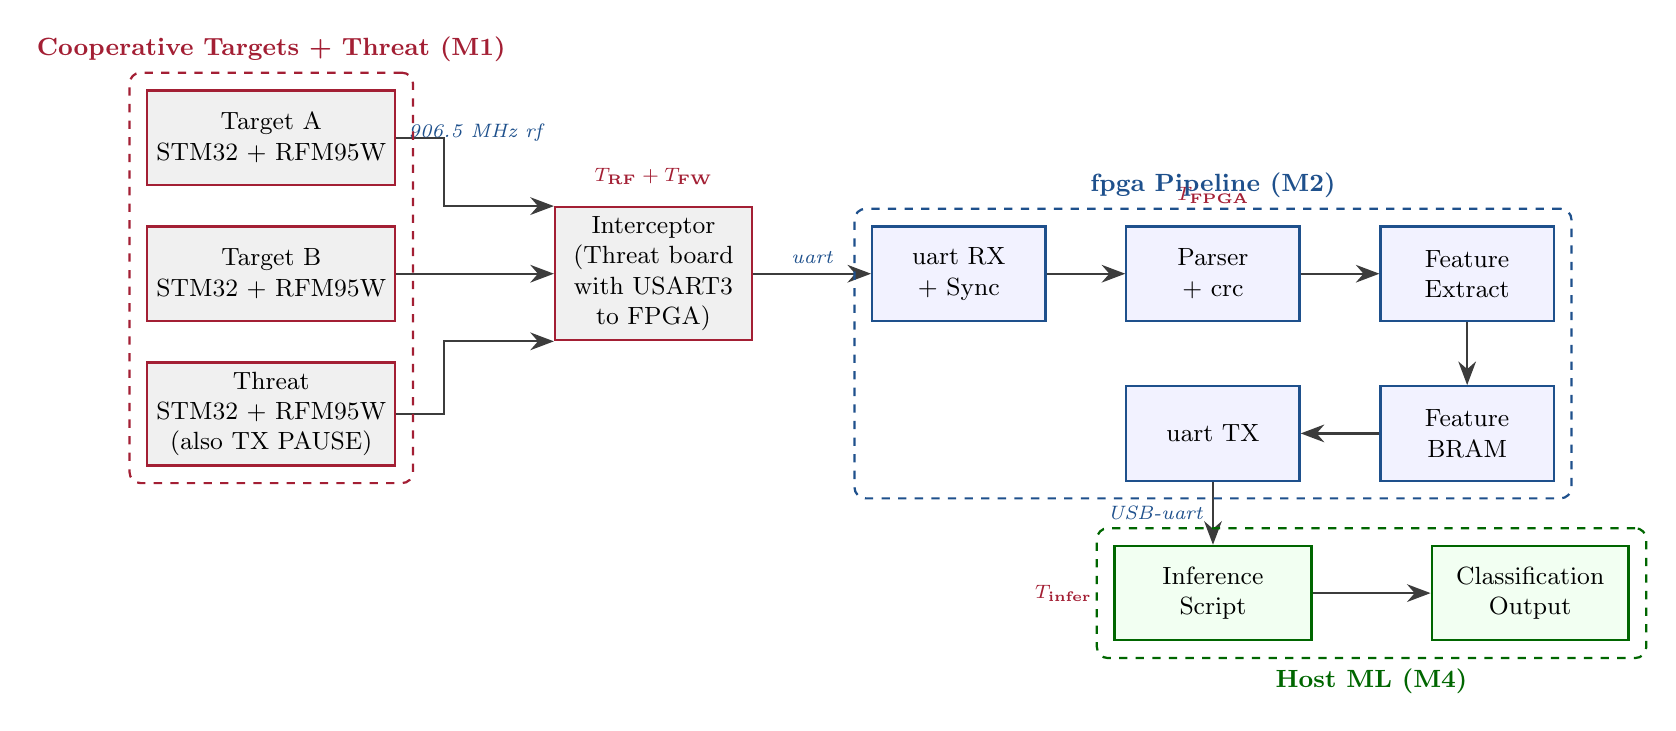
\begin{tikzpicture}[
				node distance=1cm and 1.5cm,
				hw/.style={rectangle, draw=stevens, fill=lightgray, thick,
					minimum width=2.5cm, minimum height=1.2cm, align=center, font=\small},
				fpgablk/.style={rectangle, draw=accentblue, fill=blue!5, thick,
					minimum width=2.2cm, minimum height=1.2cm, align=center, font=\small},
				swblk/.style={rectangle, draw=green!40!black, fill=green!5, thick,
					minimum width=2.5cm, minimum height=1.2cm, align=center, font=\small},
				arrow/.style={-{Stealth[length=3mm]}, thick, color=darkgray},
				elabel/.style={font=\scriptsize\itshape, color=accentblue},
				tlabel/.style={font=\scriptsize\bfseries, color=stevens}
				]

				% Cooperative targets + Threat
				\node[hw] (b1) {Target~A\\STM32 + RFM95W};
				\node[hw, below=0.5cm of b1] (b2) {Target~B\\STM32 + RFM95W};
				\node[hw, below=0.5cm of b2] (b3) {Threat\\STM32 + RFM95W\\(also TX PAUSE)};

				% Interceptor (== Threat board, FPGA feeder)
				\node[hw, right=2cm of b2] (rx) {Interceptor\\(Threat board\\with USART3\\to FPGA)};

				% FPGA pipeline
				\node[fpgablk, right=1.5cm of rx] (uart_rx) {\UART{} RX\\+ Sync};
				\node[fpgablk, right=1cm of uart_rx] (parser) {Parser\\+ \CRC{}};
				\node[fpgablk, right=1cm of parser] (feat) {Feature\\Extract};
				\node[fpgablk, below=0.8cm of feat] (bram) {Feature\\BRAM};
				\node[fpgablk, below=0.8cm of parser] (uart_tx) {\UART{} TX};

				% Host ML
				\node[swblk, below=0.8cm of uart_tx] (infer) {Inference\\Script};
				\node[swblk, right=1.5cm of infer] (display) {Classification\\Output};

				% RF arrows
				\draw[arrow] (b1.east) -- ++(0.6,0) |- (rx.north west);
				\draw[arrow] (b2.east) -- (rx.west);
				\draw[arrow] (b3.east) -- ++(0.6,0) |- (rx.south west);

				% Pipeline arrows
				\draw[arrow] (rx.east) -- (uart_rx.west) node[midway, above, elabel] {\UART{}};
				\draw[arrow] (uart_rx) -- (parser);
				\draw[arrow] (parser) -- (feat);
				\draw[arrow] (feat) -- (bram);
				\draw[arrow] (bram) -- (uart_tx);
				\draw[arrow] (uart_tx) -- (infer) node[midway, left, elabel] {USB-\UART{}};
				\draw[arrow] (infer) -- (display);

				% RF label
				\node[font=\scriptsize\itshape, color=accentblue] at ($(b1.east)!0.5!(rx.north west)+(0,0.5)$) {906.5~MHz \RF{}};

				% Timing labels
				\node[tlabel, above=0.15cm of rx] {$T_{\text{RF}} + T_{\text{FW}}$};
				\node[tlabel, above=0.15cm of parser] {$T_{\text{FPGA}}$};
				\node[tlabel, left=0.15cm of infer] {$T_{\text{infer}}$};

				% Grouping boxes
				\node[draw=stevens, dashed, thick, rounded corners,
				fit=(b1)(b2)(b3),
				inner sep=6pt,
				label={[font=\small\bfseries\color{stevens}]above:Cooperative Targets + Threat (M1)}] {};

				\node[draw=accentblue, dashed, thick, rounded corners,
				fit=(uart_rx)(parser)(feat)(bram)(uart_tx),
				inner sep=6pt,
				label={[font=\small\bfseries\color{accentblue}]above:\FPGA{} Pipeline (M2)}] {};

				\node[draw=green!40!black, dashed, thick, rounded corners,
				fit=(infer)(display),
				inner sep=6pt,
				label={[font=\small\bfseries\color{green!40!black}]below:Host ML (M4)}] {};
			\end{tikzpicture}%
		}
		\caption{Complete validated system architecture. Module labels (M1--M4) indicate which module developed each subsystem. Module~3 validated the interfaces between subsystems. Module~5 characterized the end-to-end behavior under stress. Timing labels show the latency decomposition from Section~\ref{sec:benchmark}.}
		\label{fig:final_system}
	\end{figure}

	\newpage
	% ══════════════════════════════════════════════════════════════
	\section{Hardware and Software Reference}
	\label{sec:hw_sw}
	% ══════════════════════════════════════════════════════════════

	\begin{table}[ht!]
		\centering
		\caption{Required hardware and software for Module 5.}
		\label{tab:hw_sw}
		\renewcommand{\arraystretch}{1.3}
		\begin{tabularx}{\textwidth}{l l X}
			\toprule
			\textbf{Item} & \textbf{Qty / Version} & \textbf{Purpose} \\
			\midrule
			STM32 Nucleo-L476RG + RFM95W & 3 & 2 cooperative targets (Target~A, Target~B) + 1 interceptor (Threat) \\
			915~MHz Spring Antenna & 3 & \RF{} transmission/reception (operating carrier 906.5\,MHz in U.S.\ 915\,MHz ISM band) \\
			Digilent Nexys A7-100T & 1 & \FPGA{} processing platform \\
			USB Micro-B Cables & 4--5 & Power, programming, \UART{} \\
			Breadboard + Jumper Wires & --- & Inter-board connections \\
			Oscilloscope or Logic Analyzer & 1 & Response time measurement (\GPIO{} toggle); S5 PAUSE-latency 4-channel capture \\
			Tape Measure & 1 & Distance measurement for S3 and S5 RSSI-targeting test \\
			Physical Obstruction & 1 & Signal blockage for S3e \\
			\midrule
			AMD Vivado Design Suite & 2024.1+ & \ILA{} debugging, bitstream verification \\
			VS Code + STM32 extension stack & Latest & Cooperative-target / interceptor firmware (standalone STM32CubeIDE also supported) \\
			Python 3.10+ & --- & Inference script, data analysis \\
			All Module~4 Python dependencies & --- & \texttt{pandas}, \texttt{scikit-learn}, \texttt{torch}, etc. \\
			\LaTeX{} Distribution & --- & Final report typesetting \\
			Presentation Software & --- & Slides (PowerPoint, Beamer, etc.) \\
			\bottomrule
		\end{tabularx}
	\end{table}

	% ══════════════════════════════════════════════════════════════
	\section{Assessment Rubric}
	% ══════════════════════════════════════════════════════════════

	\begin{table}[ht!]
		\centering
		\caption{Module 5 assessment rubric.}
		\label{tab:rubric}
		\renewcommand{\arraystretch}{1.3}
		\begin{tabularx}{\textwidth}{X c c}
			\toprule
			\textbf{Assessment Item} & \textbf{Weight} & \textbf{Due} \\
			\midrule
			Stress Test Report (S1--S4 results, density limits, \SNR{} degradation, stability) & 20\% & Session 17 \\
			Benchmarking Report (response time decomposition, spec table, baseline comparison) & 20\% & Session 18 \\
			Failure Analysis \& Curriculum Package (failure catalog, cross-domain tracing, full package) & 25\% & Session 19 \\
			Final Report \& Presentation (15--20 page report, 20-min presentation, live demo) & 35\% & Session 20 \\
			\bottomrule
		\end{tabularx}
	\end{table}

	\newpage
	% ══════════════════════════════════════════════════════════════
	\section{Recommended Resources}
	% ══════════════════════════════════════════════════════════════

	\subsection{System Testing and Validation}

	\begin{enumerate}[leftmargin=2em]
		\item B.\ Beizer, \textit{Software Testing Techniques}, 2nd ed., Van Nostrand Reinhold, 1990. (Stress testing methodology, boundary analysis, combinatorial testing.)
		\item J.\ A.\ Whittaker, \textit{Exploratory Software Testing}, Addison-Wesley, 2009. (Structured approaches to finding system-level failures.)
		\item IEEE Std 829-2008, ``Standard for Software and System Test Documentation,'' IEEE, 2008. (Test plan, test report, and test log formats.)
	\end{enumerate}

	\subsection{Technical Writing and Presentation}

	\begin{enumerate}[leftmargin=2em]
		\item M.\ Alley, \textit{The Craft of Scientific Presentations}, 2nd ed., Springer, 2013. (Evidence-based presentation design for technical audiences.)
		\item J.\ G.\ Paradis and M.\ L.\ Zimmerman, \textit{The MIT Guide to Science and Engineering Communication}, 2nd ed., MIT Press, 2002. (Technical report structure, audience analysis, visual design.)
		\item IEEE, ``IEEE Reference Guide,'' 2024 ed. [Online]. Available: \url{https://ieeeauthorcenter.ieee.org/} (Citation format for the final report.)
	\end{enumerate}

	\subsection{Cross-Domain System Design}

	\begin{enumerate}[leftmargin=2em]
		\item N.\ Weste and D.\ Harris, \textit{CMOS VLSI Design: A Circuits and Systems Perspective}, 4th ed., Addison-Wesley, 2010. (Chapter 1: abstraction layers and cross-level design trade-offs.)
		\item E.\ A.\ Lee and S.\ A.\ Seshia, \textit{Introduction to Embedded Systems: A Cyber-Physical Systems Approach}, 2nd ed., MIT Press, 2017. (Cross-domain modeling of embedded systems spanning hardware, firmware, and software.)
		\item A.\ G\'eron, \textit{Hands-On Machine Learning with Scikit-Learn, Keras, and TensorFlow}, 3rd ed., O'Reilly, 2022. (Chapter 2: end-to-end ML project pipeline---relevant for the final report's system-level perspective.)
	\end{enumerate}

	\subsection{Project-Specific References}

	\begin{enumerate}[leftmargin=2em]
		\item Semtech, ``SX1276/77/78/79 Datasheet,'' Rev.\ 7, 2020.
		\item STMicroelectronics, ``STM32L476xx Reference Manual,'' RM0351, Rev.\ 9, 2023.
		\item Digilent, ``Nexys A7 Reference Manual,'' Rev.\ C, 2022.
		\item Xilinx/AMD, ``Artix-7 FPGAs Data Sheet: DC and AC Switching Characteristics,'' DS181, 2023.
	\end{enumerate}

	\newpage
	% ══════════════════════════════════════════════════════════════
	\section{Framework Retrospective}
	% ══════════════════════════════════════════════════════════════

	This section provides a closing reflection on the five-module framework as a whole, intended for inclusion in the final report's Discussion section.

	\subsection{Cross-Module Dependency Summary}

	The following table summarizes the primary cross-module dependencies that shaped the system's behavior. Each row identifies a design decision, the module where it was made, and the modules where its consequences were felt.

	\begin{table}[ht!]
		\centering
		\caption{Key cross-module design dependencies.}
		\label{tab:dependencies}
		\renewcommand{\arraystretch}{1.3}
		\begin{tabularx}{\textwidth}{X c c X}
			\toprule
			\textbf{Design Decision} & \textbf{Made In} & \textbf{Felt In} & \textbf{Consequence} \\
			\midrule
			Radio packet format (32 bytes, packed \texttt{Modulation Code} byte) & M1 & M2, M3, M4 & Defines parser structure, feature vector, four-task classification scope (SF, mod, emitter ID, packet type). \\
			\UART{} at 115200 baud & M1 & M2, M3, M5 & Limits max frame rate to 268~fps; sets \FIFO{} sizing constraint. \\
			\CRC{}-8 polynomial (0x07) & M1/M2 & M3 & Mismatch between FW and RTL caused first integration failure. \\
			PAUSE protocol (100\,ms cadence, 500\,ms hold-off) & M1 (LH1-G) & M5 & Defines closed-loop response latency envelope ($\sim$151\,ms worst case) and recovery time ($\sim$1500\,ms). \\
			RSSI-table staleness threshold (5\,s) & M1 (LH1-G) & M5 & Determines when stale RSSI entries cause wrong-Target PAUSE selection. \\
			Feature vector format (32 bytes, 8 features + bit-fields) & M2 & M4, M5 & Determines classifier input dimensionality; \texttt{pkt\_type} bit-field at offset~3 enables the packet-type classification task. \\
			\FIFO{} depth (64 entries) & M2 & M3, M5 & Constrains burst tolerance; overflow under high station density + PAUSE bursts. \\
			Training data regime coverage (clean vs.\ contended) & M3 & M4, M5 & Classifier accuracy collapses outside training distribution; LH4-F operating-condition shift quantifies the gap. \\
			Stratified train/test split keyed on \texttt{run\_id} & M3 & M4 & Ensures fair evaluation; prevents within-run leakage. \\
			Label leakage prevention (esp.\ \texttt{pkt\_type}) & M4 & M4, M5 & Forces classifier to learn signal properties, not self-reported fields; the packet-type task is the most aggressive trap. \\
			\bottomrule
		\end{tabularx}
	\end{table}

	\subsection{The Framework's Central Lesson}

	\begin{tcolorbox}[infobox={Why Cross-Domain Integration Is the Subject---Not the Obstacle}]
		In a traditional curriculum, students learn \RF{} design, digital logic, embedded firmware, and machine learning as separate subjects. Each course validates student work within its own domain: firmware is tested against a simulated peripheral, \VHDL{} is verified in simulation, classifiers are trained on clean benchmark datasets. The interfaces between domains---the places where firmware decisions constrain hardware behavior, where hardware decisions shape data characteristics, where data characteristics determine \ML{} outcomes---are treated as implementation details rather than learning objectives.

		This framework inverts that relationship. The interfaces are the learning objectives. The radio packet format with its packed \texttt{Modulation Code} byte is not just a firmware deliverable---it is a data contract that propagates through three downstream modules and unlocks a fourth classification task that would not otherwise exist. The \FPGA{} feature vector is not just a digital design exercise---it is the sole information bridge between the physical \RF{} world and the statistical \ML{} world. The training dataset is not just a collection of numbers---it is an empirical sample of a physical system whose distribution (clean vs.\ contended regime) is shaped by every hardware and firmware decision that preceded it. The PAUSE protocol is not just a stress-test feature---it is the framework's most explicit demonstration that intercept-and-act behavior requires every disciplinary domain to cooperate.

		The student who completes this framework has not merely built a system that classifies \RF{} signals. They have experienced---through direct, sometimes painful encounter with integration failures---the reality that engineering systems are defined by their interfaces, not their components.
	\end{tcolorbox}

	\vfill
	\clearpage
	\printnoidxglossary[type=\acronymtype,title={Glossary}]

	\begin{center}
		\rule{0.5\textwidth}{0.4pt}\\[6pt]
		{\small\textcolor{darkgray}{End of Module 5 Lesson Plan}}
	\end{center}

\end{document}
